
\section{Aufbau}
\label{sec:Versuchaufbau}

Der verwendete Versuchsaufbau nutzt als Photonenquelle eine Spektrallampe (siehe Abbildung \ref{fig:Versuchsaufbau}).
Das Licht wird, um nur $D_1$-Licht zu erhalten, durch eine Sammellinse fokussiert und daraufhin die entsprechende Wellenlänger heraus gefiltert.
Mit einem $\lambda /4$-Plättchen wird eine Phasenverschiebung von $\pi /2$ erzeugt, wodurch das zuvor linear polarisierte Licht rechtszirkular polarisiert wird.
Das Licht trifft dann auf eine Dampfzelle in der sich das $\ce{^{87}_{}Rb}$ und $\ce{^{85}_{}Rb}$-Gas befindet.
Um diese Zelle herum befinden sich drei Helmholtz-Spulenpaare, eine Horizontalfeld-Spule, eine horizontale Modulationsfeldspule und eine Vertikalfeld-Spule.
Die Hochfrequenzstrahlung wird mit einer RF-Spule erzeugt.
Danach wird das Licht auf eine Si-Doide fokussiert, die die Intensität bestimmt und auf einem angeschlossen  Oszilloskop dargestellt.

\begin{figure}
 \centering
 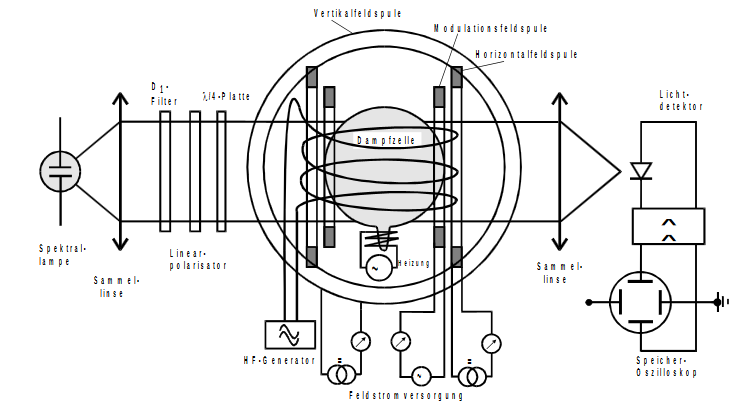
\includegraphics[width=0.8\textwidth]{img/Aufbau.png}
 \caption{Versuchsaufbau. \cite{skript}}
 \label{fig:Versuchsaufbau}
\end{figure}
